% xetex compatible variant that support TTF fonts according to company rules
\documentclass[ignorenonframetext, professionalfonts, hyperref={unicode}]{beamer}

\usetheme{Epam}

\usepackage{fontspec}
\setsansfont{SourceSansPro-Regular}
%\setbeamerfont{frametitle}{family=\fontspec{Oswald}}
\setbeamerfont{frametitle}{family=\fontspec{Oswald}}
\setbeamerfont{block title}{family=\fontspec{Oswald}}

%\setmainfont{Times New Roman}
\defaultfontfeatures{Mapping=tex-text}
\defaultfontfeatures{Ligatures=TeX}

%\setsansfont{Arial}
%\setromanfont{Trebuchet MS}

\usepackage{cmap}
\usepackage{graphicx}

\usepackage{textcomp}

\usepackage{beamerthemesplit}

\usepackage{ulem}

\usepackage{verbatim}
\usepackage{import}

\usepackage{listings}
\lstloadlanguages{bash}

\lstset{escapechar=`,
	captionpos=b,
	extendedchars=false,
	language=sh,
%	frame=single,
	tabsize=2, 
	columns=fullflexible, 
%	basicstyle=\scriptsize,
	keywordstyle=\color{blue}, 
	commentstyle=\itshape\color{brown},
%	identifierstyle=\ttfamily, 
	stringstyle=\mdseries\color{green}, 
	showstringspaces=false, 
	numbers=left, 
	numberstyle=\footnotesize, 
	breaklines=true, 
	inputencoding=utf8,
	keepspaces=true,
	morekeywords={u\_short, u\_char, u\_long, in\_addr}
	}

\definecolor{darkgreen}{cmyk}{0.7, 0, 1, 0.5}

\lstdefinelanguage{diff}
{
    morekeywords={+, -},
    sensitive=false,
    morecomment=[l]{//},
    morecomment=[s]{/*}{*/},
    morecomment=[l][\color{darkgreen}]{+},
    morecomment=[l][\color{red}]{-},
    morestring=[b]",
}

\author[Epam]{{\bf Epam}\\Low Level Programming Department}

%\institution[EPAM]{EPAM}
%\logo{\includegraphics[width=1cm]{logo.png}}

\graphicspath{{../../slides/cmdline/clipart/}{../../slides/bash/clipart/}}

\bibliographystyle{unsrt}
\setbeamertemplate{bibliography item}{\insertbiblabel}

\AtBeginSection[]{%
  \begin{frame}<beamer>
    \frametitle{}
    \tableofcontents[
        sectionstyle=show/shaded, hideallsubsections ]
  \end{frame}
  \addtocounter{framenumber}{-1}% If you don't want them to affect the slide number
}

% \regex for regular expressions
\newcommand{\regex}[1]{ %
\expandafter{$\ulcorner{\color{blue}\texttt{#1}}\lrcorner$} %
}


%\title[bash]{Bourne again shell}
\title{Введение в GNU/Linux}

%%%%%%%%%%%%%%%%%%%%%%%%%%%%%%%%%%%%%%%%%%%%%%%%%
%%%%%%%%%% Begin Document  %%%%%%%%%%%%%%%%%%%%%%
%%%%%%%%%%%%%%%%%%%%%%%%%%%%%%%%%%%%%%%%%%%%%%%%%

\begin{document}

\begin{frame}
	\frametitle{BASH}
	\titlepage
	\vspace{-0.5cm}
	\begin{center}
	%\frontpagelogo
	\end{center}
\end{frame}

\begin{frame}
	\tableofcontents
%	[hideallsubsections]
\end{frame}



%%%%%%%%%%%%%%%%%%%%%%%%%%%%%%%%%%%%%%%%%   
%%%%%%%%%% Content starts here %%%%%%%%%%
%%%%%%%%%%%%%%%%%%%%%%%%%%%%%%%%%%%%%%%%%

\section{Configure network settings}
\mode<all>{\begin{frame}{Сетевая подсистема Linux}

	\begin{block}{Cетевой интерфейс}

		Сетевой интерфейс в Linux -– это абстрактный \alert{именованный} объект,  используемый для передачи 
		данных через некоторую линию связи без привязки к ее (линии связи) реализации.
	\end{block}
\end{frame}

\begin{frame}{Сетевая подсистема Linux}

	\center\includegraphics[width=0.9\textwidth]{../../slides/networking/06-netstack.png}

\end{frame}


} % add real config

\subsection{Управление интерфейсами}
\mode<all>{\input{../../slides/networking/interface-management}}

\subsection{Полезные программы}
\mode<all>{\begin{frame}{Полезные утилиты}
	\begin{center}
		\begin{itemize}
			\item netstat / ss
			\item nslookup / dig
			\item ping
			\item traceroute
			\item tcpdump
			\item telnet
			\item netcat
			\item nmap
		\end{itemize}
	\end{center}

\end{frame}


%\begin{frame}{Полезные утилиты: практика}
%
%	\begin{columns}
%		\column{0.5\textwidth}
%		\begin{block}{netstat}
%
%			Узнать:
%			\begin{itemize}
%				\item список используемых сокетов
%				\item серверных сокетов
%				\item имена/pid серверов
%				\item узнать номера портов
%			\end{itemize}
%		\end{block}
%	
%		\pause
%		\column{0.5\textwidth}
%		\begin{block}{telnet/netcat}
%
%			\begin{itemize}
%				\item Чат по протоколу TCP с соседом
%				\item Чат по протоколу UDP с соседом
%				\item Передать текстовый и бинарный файлы
%			\end{itemize}
%	
%			При создании чата использовать {\tt netstat} и {\tt tcpdump}
%			для получения информации о соединении.
%		\end{block}
%	
%	\end{columns}
%\end{frame}
%
%nmap
%1. сканирование соседа
%2. сканирование выделенных портов у соседа (поиск сервера чата) 
%3. узнать список открытых портов на всех машинах в 505
%4. узнать список  работающих машин
%
%tcpdump
%0. pcap файлы/libpcap
%1. запуск монитора
%2. запуск чата
%3. монитор-фильтр-анализ
%
}

\subsection{Маршрутизация}
\mode<all>{\input{../../slides/networking/routing}}

\section{Write and run shell script}
\mode<all>{\begin{frame}{Преимущества автоматизации для сложных задач}
    \begin{center}
      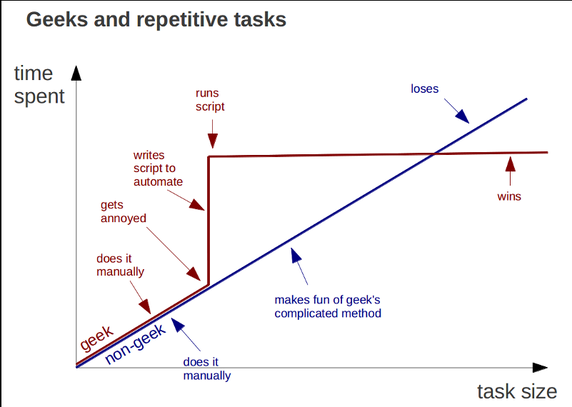
\includegraphics[width=3.6in]{view_automate_geek_vs_nongeek}
    \end{center}
\end{frame}

}
\mode<all>{\begin{frame}[fragile]{Оболочка операционной системы}

     \begin{block}{Оболочка операционной системы}
     (от англ. shell «оболочка») \alert{интерпретатор команд} операционной системы, обеспечивающий интерфейс для взаимодействия пользователя с функциями системы.  
     \end{block}

     Что такое Unix shell?
     \begin{itemize}
        \item Обычная программа, запускающаяся после входа в систему
	\pause
        \item Интерактивный командный интерпретатор
	\pause
        \item Платформа интеграции для утилит (glue-language)
	\pause
        \item Язык программирования
	\pause
        \item Макропроцессор (программа выполяняющая преобразование текста)
     \end{itemize}

        Например:
	\pause
	Оболочки из Windows --  cmd.exe, PowerShell

	Минимальный дистрибутив Linux -- ядро + shell 

\end{frame}
}
\mode<all>{\begin{frame}[fragile]{Задание. Виды оболочек.}
Получить список установленных оболочек.
\begin{lstlisting}[language=bash]
cat /etc/shells
ls -l <filename> # для каждого элемента /etc/shells
readlink -e <filename> 
\end{lstlisting}
Запустить любую из установленных оболочек. 

\begin{lstlisting}[language=bash]
/usr/bin/ksh 
/usr/bin/zsh 
/usr/bin/fish
\end{lstlisting}

\alert{Bash} - (Bourne-again shell) оболочка по умолчанию в большинстве дистрибутивов Linux.

выход из оболoчки  Ctrl-D, либо exit
\end{frame}
}
\mode<all>{\begin{frame}
  \frametitle{Bash против скриптовых языков}
  \begin{itemize}
   \item В bash трудно делать сложные структуры данных
   \item В bash нет типизации переменных
   \item Но! В bash очень просто организовывать взаимодействие внешних программ
   \item Stream programming \texttt{(a | b | c )}
  \end{itemize}
\end{frame}

\begin{frame}
  \frametitle{Когда использовать bash}
  \begin{columns}
   \column{0.5\textwidth}
    \begin{center}
     {\Large Использовать}
    \end{center}
    \begin{itemize}
      \item Прототипирование
      \item Системные скрипты, обертки
      \item Автоматизация консоли
    \end{itemize}
   \column{0.5\textwidth}
    \begin{center}
     {\Large Не использовать}
    \end{center}
    \begin{itemize}
      \item Критичные по скорости (интерпретатор)
      \item GUI
      \item Сложные структуры данных (двумерный массив, бинарные деревья, нет типизации переменных)
    \end{itemize}
  \end{columns}
\end{frame}
}
\mode<all>{\begin{frame}[fragile]{Запуск программы из командной строки}
  \begin{itemize}
    \item 
	Находим приглашение командной строки
	\$, \#, user@host:~\$
    \item
	Вводим имя команды, аргументы и запускаем на выполнение нажатием <Enter>
   \end{itemize}

	Что такое команды?
  \begin{itemize}
    \item исполняемая программа (бинарный файл, скрипт)
    \item встроенные в оболочку команды (shell built-ins)
    \item функция оболочки
    \item сокращение команды (an alias) 
  \end{itemize}
\end{frame}
}
\mode<all>{\begin{frame}[fragile]{Задание. Виды команд в оболочке}
Команда  \alert{type} отображает тип команды. Выполним ее для различных команд.
\begin{lstlisting}[language=bash]
type type cd help alias read
type dmesg rm
type if
type -a ls
type -a echo pwd test
\end{lstlisting}
Два типа команд. А оно нам надо? Есть ли разница?
\pause
Встроенные и внешние команды
\begin{itemize}
    \item всегда присутствуют в интерпретаторе, внешних может и не быть на диске
    \item однообразный синтаксис на разных платформах (переносимость скриптов)
    \item как правило выполняются быстрее, т.к. код находится в памяти
    \item есть средства, чтобы выключить встроенные команды, либо использовать прямой путь
\end{itemize}
\end{frame}
}
\mode<all>{\begin{frame}[fragile]
  \frametitle{Скрипты}
 
  \begin{block}<1->{Shell Script, определение}  

    Последовательность команд Shell.

    Разделитель: перевод строки, \textquotedbl ; \textquotedbl
  \end{block}

  \begin{block}<2->{shebang}
    \verb+#!something+ или чем мы запускаем скрипт. 
    
    По умолчанию : \verb+#!/bin/sh+
  
    Всегда первая строка скрипта.

    Фактически: \verb+/bin/sh scriptname+
  \end{block}

  \begin{block}<3->{Парадоксальные примеры}
    \verb+#!/bin/rm+

    \verb+#!/bin/awk -f+

    \verb+#!/bin/less+
  \end{block}

\end{frame}
}
\mode<all>{\begin{frame}[fragile]
  \frametitle{Запуск скриптов}
  \begin{enumerate} 
    \item \verb+sh scriptname+
    \item \verb-chmod +x script- \newline \verb+./script+
    \item из каталогов в переменной PATH 
      \newline \verb+echo $PATH+
      \newline \verb+~/bin+ (если есть)
      \newline \verb+/usr/local/bin+
    \item в текущей копии shell\footnote{ Остальные способы - запускают новый shell}
      \newline \verb+. ./script+
      \newline \verb+source script+\footnote{ Несовместимо с POSIX. Происходит из ksh. Добавляет текущий каталог к списку путей}
  \end{enumerate}
\end{frame}
}

\section{Manipulate the different I/O streams  with I/O Redirection}
\mode<all>{\begin{frame}[fragile]
	\frametitle{stdin, stdout, stderr}
     C каждым процессом связаны потоки ввода-вывода - файловые дeскрипторы stdin, stdout, stderr.
    \begin{block}{Пример. Номера файловых дeскрипторов и устройств. }
                    \begin{lstlisting}
echo /dev/std*
echo /dev/std* | xargs -t -n 1 readlink
lsof -ap $BASHPID -d 0,1,2
                    \end{lstlisting}
    \end{block}
\end{frame}
}
\mode<all>{

\begin{frame}{Конвееры}
%  \textbf{Цель} -- максимальная модульность: большое количество простых приложений, взаимодействующих друг с другом для решения задач
  \only<1>{
  \begin{center}
    \includegraphics[width=1.2in]{../../slides/cmdline/process}
  \end{center}
  }
  \only<2>{
    \begin{center}
      \includegraphics[width=3.6in]{../../slides/cmdline/processes}
    \end{center}
  }
  \begin{itemize}
    \item <1-> Каждое приложение открывает 3 стандартных файловых дескриптора (file descriptor) \alert{stdin (fd 0)}, \alert{stdout(fd 1)}, \alert{stderr (fd 2) }
    \item <2-> Приложения могут работать как фильтр из \alert{STDIN} в \alert{STDOUT}, можно объединять несколько приложений в конвейер
    \item <2-> Синтаксис {\tt <app1> | <app2>}
  \end{itemize}
\end{frame}
}
\mode<all>{\begin{frame}{Перенаправления в файл}

\begin{itemize}
  \item Перенаправление stdout FD=1
    \begin{itemize}
      \item С созданием нового файла

        {\tt command > file}\\
		Например {\tt cat file1 file2 > file3}
      \item С дополнением существующего

		  {\tt command >\phantom{}>  file}
    \end{itemize}
    \pause
  \item Перенаправления stdin FD=0

    {\tt command < file}
    \pause
  \item Перенаправления stderr FD=2

    {\tt command1 2>\&1 | command2}

   {\tt command 1>file 2>\&1}

   {\tt command 2>file 1>\&2}
\end{itemize}

\end{frame}
}
\mode<all>{\begin{frame}{Применение перенаправления потоков.}
Работает с любым типом файлов.
\begin{itemize}
  \item Создать новый файл или обнулить сущствующий >
  \item Перенаправить длинный вывод команды в файл >
  \item Молчаливое выполнение команды >/dev/null 
  \item Чтение из спецфайла </dev/urandom, /dev/zero 
  \item Чтение из данных из файла <
  \item Настройка системы. echo >  определенные файлы в /proc/ или /sys/
  \item cat /dev/zero > /dev/sda - удалить систему
\end{itemize}

\end{frame}
}
%\mode<all>{\begin{frame}[fragile]
	\frametitle{Перенаправление ввода/вывода}

	\begin{itemize}
		\item ``>'' -- Перенаправление в файл
			\begin{block}{Пример}
				\begin{lstlisting}
echo stdout > test.txt
				\end{lstlisting}
			\end{block}
		\item ``>\&'' -- Перенаправление в другой дескриптор
			\begin{block}{Пример}
				\begin{lstlisting}
(echo stdout; echo stderr >&2) > test.txt
				\end{lstlisting}
			\end{block}
	\end{itemize}

\end{frame}
}
%\mode<all>{\begin{frame}[fragile]
	\frametitle{Перенаправление ввода/вывода}

	\begin{itemize}

		\item ``\&>''
			\begin{block}{Пример}
				\begin{lstlisting}
(echo stdout; echo stderr >&2) &> test.txt
\end{lstlisting}
			\end{block}
		
		\item ``>{}>'' -- Добавление в файл
			\begin{block}{Пример}
				\begin{lstlisting}
echo stdout >> test.txt
\end{lstlisting}
			\end{block}

		\item ``<'' -- Чтение из файла
			\begin{block}{Пример}
				\begin{lstlisting}
cat < test.txt
\end{lstlisting}
			\end{block}
	\end{itemize}

\end{frame}
}
%\mode<all>{\begin{frame}[fragile]
	\frametitle{Перенаправление ввода/вывода}

	\begin{itemize}

		\item ``<<'' -- Here-документ

		\item ``<>'' -- Открывает файловый дескриптор из файла/другого дескритора
			\begin{block}{Пример}
				\begin{lstlisting}
exec 3<>test.txt; echo test >&3;  cat <test.txt
				\end{lstlisting}
			\end{block}
			
		\item ``n<\&-'' -- Закрывает файловый дескриптор
			\begin{block}{Пример}
				\begin{lstlisting}
exec 3<&-; echo test >&3
				\end{lstlisting}
			\end{block}
			
		\item ``|'' -- pipe
	\end{itemize}

\end{frame}
}

%\mode<all>{\begin{frame}[fragile]
	\frametitle{Начало скрипта \#!}

        Конструкция позволяет использовать скрипты, как системные команды. 
        Первая cтрока игнорируется интерпретатором, т.к. \# - комментарий

	\begin{block}{Sha-Bang, shebang, hasbang}
		\begin{lstlisting}
#!/bin/bash
		\end{lstlisting}
	\end{block}

	\begin{block}{Режим совместимости с POSIX}
		\begin{lstlisting}
#!/bin/sh
		\end{lstlisting}

	\end{block}

\end{frame}
}

\section{Understand expansion}
% bash macroprocessor
\mode<all>{\begin{frame}{Встроенный макропроцессор}

\begin{itemize}
    \item brace expansion  \alert{\{ \}} фигурные скобки
    \item tilde expansion \alert{\textasciitilde{}file}
    \item parameter and variable expansion \alert{\$name}, \alert{\$\{name\}} 
    \item command substitution \alert{\$( )} круглые скобки
    \item arithmetic expansion \alert{(())}, \alert{\$(())} двойные круглые скобки
    \item word splitting \alert{"}, \alert{'}, \alert{\textvisiblespace} пробел
    \item filename expansion (globbing) \alert{*}, \alert{?}, \alert{[]} 
\end{itemize}
    
\end{frame}
}
% brace expansion
\mode<all>{\begin{frame}
	\frametitle{Спецсимвол фигурная скобка}

	\begin{block}{Фигурные скобки и склеивание с помощью ``,``}
		\begin{itemize}
			\item Посмотреть на результат выполнения команды \\
				{\tt echo \{A,B,C\}:\{1,2,3\}}
				\pause
			\item Посмотреть на результат выполнения команды \\
				{\tt ls -l \{,/usr\}/\{bin,sbin\}/*sh}
		\end{itemize}
	\end{block}

	\pause

	\begin{block}{Фигурные скобки и перечисления с помощью ``..``}
		\begin{itemize}
			\item Посмотреть на результат выполнения команды \\
				{\tt echo \{a..d\}:\{-10..10\}}
		\end{itemize}
	\end{block}

\end{frame}

\begin{frame}{Спецсимвол фигурная скобка}

Применяют как простой генератор строк и последовательностей
\begin{itemize}
    \item в циклах 
    \item для создания вложенных директорий 
    \item генерации файлов по шаблону. Файл не обязательно существует на в файловой системе.
\end{itemize}
    
\end{frame}
}
% tilde expansion
\mode<all>{\begin{frame}[fragile]{Подстановка - домашняя директория}

\begin{lstlisting}
echo ~
echo ~/.ssh
echo $HOME/.ssh
echo ~test01/.ssh/
\end{lstlisting}

\pause
\begin{itemize}
    \item \textasciitilde{} - сокращение \$HOME 
    \item \textasciitilde{}user/ - \$HOME для пользователя user
    \item / - символ завершает действие \textasciitilde{} 
\end{itemize}

Широко применяется в скриптах, на страницах документации
    
\end{frame}
}
% parameters expansion
\mode<all>{\begin{frame}
	\frametitle{Специальные параметры}

	Позиционные параметры - передаются при запуске скрипта, средство передачи данных в скрипт.

        Например: 

        ./myscript.sh file.txt /tmp/

        \$1 file.txt

        \$2 /tmp/
        
	\begin{itemize}
		\item \$0-9, \$\{10\}.. -- значение соответствующего параметра
		\item \$\# -- количество переданных параметров
		\item \$* -- представляется, как одна строка
		\item \$@ -- каждый параметр, как отдельная строка
	\end{itemize}

\end{frame}


\begin{frame}[fragile]
	\frametitle{shift}

	Встроенная команда сдвига параметров влево.

        По умолчанию сдвигает на один параметр.

	В качестве параметра может принимать число -- на сколько параметров сдвигать.

\begin{lstlisting}
shift [num]
\end{lstlisting}

\end{frame}


% \begin{frame}
%	\frametitle{Задание}
%
%	\begin{enumerate}
%		\item Написать скрипт,  который выдает количество переданных параметров
%			\pause
%		\item Вывести на экран имя команды
%			\pause
%		\item Сделать symlink на скрипт и запустить
%			\pause
%		\item Вывести на экран первых 3 параметра
%			\pause
%		\item Передать строку "I am user \$USER" в качестве параметра
%			\begin{itemize}
%				\item Без экранирования
%				\item С экранированием ''
%				\item С экранированием '
%			\end{itemize}
%			\pause
%		\item Добавить shift перед выводом параметров
%	\end{enumerate}
%\end{frame}
%

}
% globbing
\mode<all>{\begin{frame}[fragile]
	\frametitle{Задание. Строка спецсимволов}
Вывести символ * 10 раз.
				\begin{lstlisting}
echo *********
                                \end{lstlisting}
\end{frame}
}
\mode<all>{\begin{frame}[fragile]
  \frametitle{Подстановочные символы путей (globbing)}

  \alert{Wildcard characters} - спецсимволы в параметрах команд, раскрываемые в путь и имя файла самим интерпретатором перед тем, как запустить команду на выполнение. \pause


  \begin{itemize}
    \item \alert{*} - любое количество любых символов
\begin{lstlisting}[basicstyle=\normalsize]
        echo *
        ls /u*
\end{lstlisting} \pause
    \item \alert{[]} - символ из перечисления\footnote{об интервалах - в разделе о регулярных выражениях}
\begin{lstlisting}[basicstyle=\normalsize]
        echo .[bp]*
        ls /sys/*/net/
\end{lstlisting} \pause
    \item \alert{?} - любой одиночный символ
\begin{lstlisting}[basicstyle=\normalsize]
        ~$ echo ?i*
\end{lstlisting} 
  \end{itemize}

\end{frame}

}
%command expansion
\mode<all>{\begin{frame}
	\frametitle{Подстановка команд}
	
	Синтаксис:

	\begin{itemize}
		\item \`{}command\`{}
		\item \$(command)
	\end{itemize}
	\pause
	\begin{block}{Задание}
Присвоить переменной LIST результат выполнения команды {\tt ls -1} \\
Вывести на экран переменную LIST
	\end{block}
\end{frame}
}

% spaces
\mode<all>{\begin{frame}[fragile]
	\frametitle{Задание. Обработка пробелов.}
Сравнить результаты команд для имени, которое содержит пробелы
				\begin{lstlisting}
ls a long file name with spaces
ls "a long file name with spaces" 
				\end{lstlisting}
\end{frame}
}
%IFS
\mode<all>{\begin{frame}[fragile]
  \frametitle{IFS - internal field separator}

  \alert{IFS}

  Переменная, регулирующая разделение параметров (аргументов) на слова. 
  
  Используется:
  \begin{itemize}
    \item во время раскрытия параметров командной строки перед выполнением
    \item редактирование командной строки (удаление слова, Ctrl+W)
    \item чтение ввода пользователя командной \alert{read}
  \end{itemize}

  Значение по умолчанию: \textquotedbl <пробел><табуляция><перевод строки> \textquotedbl


\end{frame}
}

% symbols escape
\mode<all>{\begin{frame}[fragile]
	\frametitle{Экранирование}

	\begin{columns}
		\column{0.5\textwidth}
		\begin{itemize}
			\item Экранирование одного символа \alert{ \textbackslash }
			\item Частичное экранирование \alert{ '' }
			\item Полное экранирование \alert{ ' }
		\end{itemize}
		\pause
		\column{0.5\textwidth}
		Спецзначения для echo и sed
		\begin{itemize}
			\item \textbackslash{n} -- новая строка
			\item \textbackslash{r} -- возврат каретки
			\item \textbackslash{t} -- табуляция
			\item \textbackslash{v} -- вертикальная табуляция \\
				\small\begin{lstlisting}
echo -e "test \v test \v test"
				\end{lstlisting}
			\item \textbackslash{b} -- перемещение на 1 символ назад
			\item \textbackslash{a} -- звуковой сигнал
			\item \textbackslash{0xxx} -- 8-миричное число
			\item \textbackslash{xXX} -- 16-ричное число
		\end{itemize}
	\end{columns}

\end{frame}
}
%comments
\mode<all>{\begin{frame}
	\frametitle{Спецсимволы}

	\begin{itemize}
		\item \# -- Вся строка после \# является комментарием
		\item ; -- Разделение команд
		\item : -- NOP оператор (похож на встроенный вызов true)
		\item {\tt source} или {\bf .} -- скрипт выполняется в текущем экземпляре shell
	\end{itemize}

\end{frame}
}
\mode<all>{\begin{frame}[fragile]
	\frametitle{Запуск группы команд в Subshell.}
	
	\begin{block}{Пример}
\begin{lstlisting}
( echo 1; echo 2) | tee file
\end{lstlisting}
	\end{block}
	\begin{block}{( cmd1; cmd2)}
	    Запускается новый shell
	\end{block}
\end{frame}

\begin{frame}[fragile]
	\frametitle{Примеры использования Subshell.}
	\begin{block}{Пример. Сохраняем директорию.}
\begin{lstlisting}
echo "$PWD"
( cd /usr; echo "$PWD" )
echo "$PWD"
\end{lstlisting}
	\end{block}
\end{frame}

\begin{frame}[fragile]
	\frametitle{Примеры использования Subshell.}
	\begin{block}{Пример. Сохраняем значение переменной TEST}
\begin{lstlisting}
TEST=42; (echo Subshell TEST=$TEST; TEST=0; echo Subshell TEST=$TEST ); echo External TEST=$TEST
\end{lstlisting}
	\end{block}
	\begin{block}{Пример. Отличие от анонимной функции.}
\begin{lstlisting}
TEST=42; { echo Subshell TEST=$TEST; TEST=0; echo Subshell TEST=$TEST ; }; echo External TEST=$TEST
\end{lstlisting}
	\end{block}
\end{frame}
}
%exit code
\mode<all>{\begin{frame}[fragile]

  \Large{\alert{Код возврата (RETURN CODE)}}: \newline 
  \normalsize{результат выполнения у любой команды Shell}
  \newline

  Shell return code:
  \begin{itemize}
    \item 0 - выполнено успешно
    \item не 0 - ошибка
    \item Код возврата доступен через переменную \$?
  \end{itemize}

	\pause
	\begin{block}{Пример}
		\begin{lstlisting}
/bin/true; echo $?
/bin/false; echo $?
		\end{lstlisting}
	\end{block}

	Скрипт возвращает код последней команды, поэтому для корректного выхода необходимо использовать команду {\tt exit 0} - в случае успеха

\end{frame}
}
%\mode<all>{\begin{frame}[fragile]
  \frametitle{Условное выполнение команд}

  \Large{\alert{Код возврата (RETURN CODE)}}: \newline 
  \normalsize{результат выполнения у любой команды Shell}
  \newline

  Shell return code:
  \begin{itemize}
    \item 0 - выполнено успешно
    \item не 0 - ошибка
  \end{itemize}
  \pause

  Операции над кодом возврата:
  \begin{itemize}
    \item \textquotedbl \verb+&&+ \textquotedbl - логическое И
    \item \textquotedbl \verb+||+ \textquotedbl - логическое ИЛИ
  \end{itemize}
  \pause

  Примеры:
  \begin{itemize}
    \item \verb+ cat /proc/1/environ || echo fail +
    \item \verb+ find /usr/share/doc -name \textquotedbl *.txt \textquotedbl && echo ok+
  \end{itemize}

\end{frame}
}

%exec
%\mode<all>{\begin{frame}
	\frametitle{exec}

	Заменяет текущий shell переданной командой. 

	Часто используется для переназначения файловых дескрипторов.

\end{frame}
}

\section{Use variables in scripts}

\mode<all>{%% Vars


\begin{frame}
	\frametitle{Переменные}
	\large\center{Нетипизированные!!!}

	Для прямого обращения необходимо использовать префикс \\
	\center{\Large{\tt \$}}

	Фигурные скобки используют для отделения от текста:\\
	\center{\tt \$VARrest != \$\{VAR\}rest}

	%\bigskip
	
	\begin{alertblock}{Используют без префикса}
		\begin{itemize}
			\item в объявлении declare var
			\item в присвоении declare var=10
			\item чтение в командe read var
			\item удаление unset var
			\item в арифметических операциях {\tt (( a=b+c ))}
		\end{itemize}
	\end{alertblock}
\end{frame}

\begin{frame}[fragile]
	\frametitle{Задание. Присвоить переменной значение.}

	\begin{lstlisting}
#!/bin/bash

VAR=string
echo $VAR
	\end{lstlisting}


	\begin{block}{Изменить и посмотреть на результат.}
		\begin{itemize}
			\item Добавить пробел до знака ''{\tt =}''
			\item Добавить пробел после знака ''{\tt =}''
			\item Присвоить переменной VAR значение: I love \$\$\$!
			\item Создать переменные с другим именем и значением var 1var \_var var1
		\end{itemize}
	\end{block}

\end{frame}

\begin{frame}[fragile]
	\frametitle{Косвенное обращение к переменной}

	Косвенное (indirect) обращение к переменной: {\tt \$\{!VARIABLE\}}

	\begin{block}{Пример}
		\begin{lstlisting}
#!/bin/bash 
num=$# 
lastarg=${!num} 
echo $num $lastarg
		\end{lstlisting}
	\end{block}

\end{frame}


\begin{frame}
	\frametitle{Типы переменных}
	\begin{itemize}
		\item Локальные\\
		    Область видимости -- текущая программа, функция или субшелл
		\item Окружения
		\item Позиционные параметры
	\end{itemize}
\end{frame}



\begin{frame}
	\frametitle{Внешние переменные}

	\center{Наследование внешней переменной}

	\begin{itemize}
		\item export
		\item Переданное в командной строке \\
			\begin{block}{Пример}
				{\tt TEST=123 make}
			\end{block}
	\end{itemize}
\end{frame}


\begin{frame}[fragile]
	\frametitle{Специальные переменные}

	Часто используемые в скриптах:

	\begin{itemize}
		\item Разделитель \$IFS
		\item Директории -- домашняя \$HOME и текущая \$PWD
		\item UID пользователя -- \$UID
		\item ID процесса -- \$\$
		\item Имя хоста -- \$HOSTNAME
		\item Вид командной строки: \$PS1 -- \$PS4
		\item Локализация
			\begin{itemize}
				\item Используемый язык \$LANG
				\item Локализация \$LC\_ALL
					\begin{block}{Пример}
						\begin{lstlisting}
ls -l 
LC_ALL=C ls -l
						\end{lstlisting}
					\end{block}
			\end{itemize}
	\end{itemize}

\end{frame}



}


\end{document}
